

\chapter{Basics}

\section{Recap Authentication}
    \begin{itemize}
        \item Integrity of messages within a closed group
        \item Authentication is symmetric: Anyone who can verify authenticated messages in the group can also authenticate
        \item Should your bank be able to authenticate transaction on behalf of you?
        \item Can we separate authentication and verification?
    \end{itemize}
    \begin{center}
	    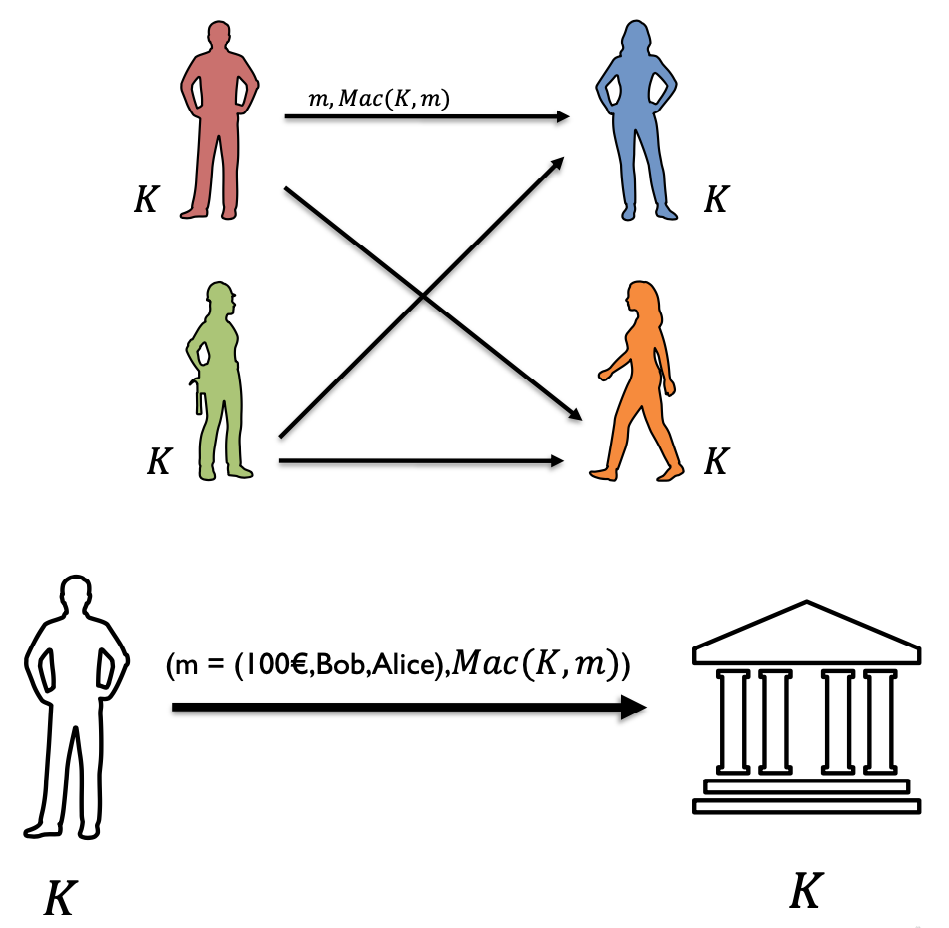
\includegraphics[width=140mm]{Graphics/Digital Signatures/ds1.png}
    \end{center}

\section{RSA Signatures}
    \begin{itemize}
        \item The notion of digital signatures was introduced by Rivest, Shamir and Adleman ’78
        \item Authentication/Signing uses a secret signing key, verification a public verification key
        \item This was the first non-encryption use of cryptography
        \item Idea: Run the textbook RSA encryption scheme in reverse
        \item Idea for Security: RSA function $m^e\ mod\ N$ hard to invert, so it shouldn’t be possibly to sign without knowledge of $sk$
    \end{itemize}
    \begin{center}
	    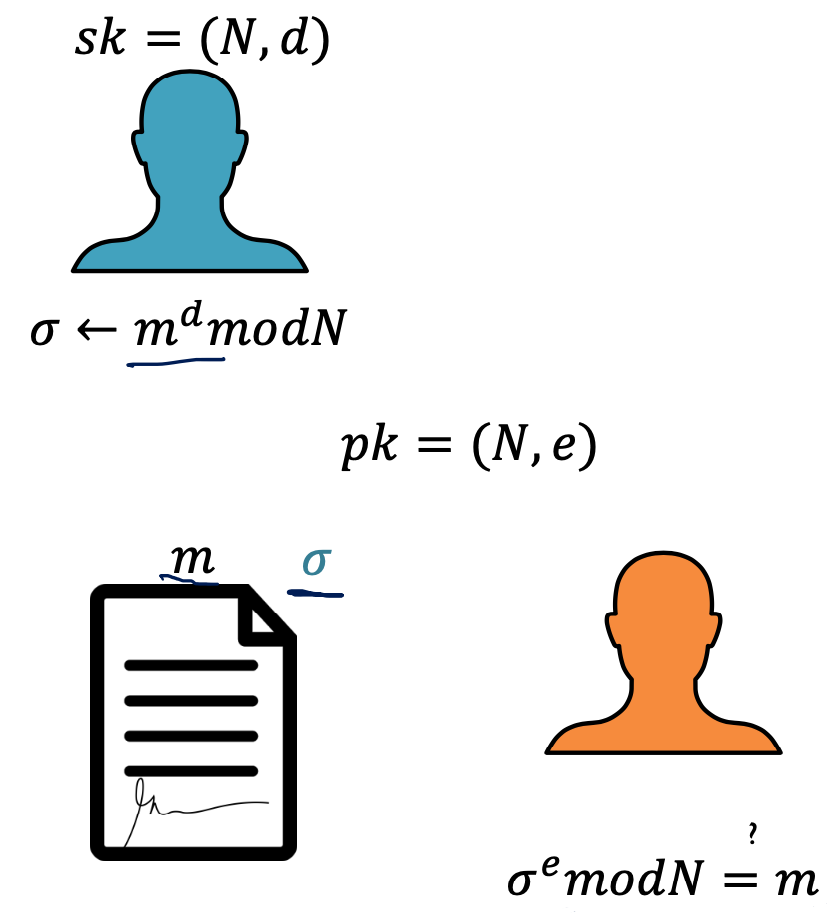
\includegraphics[width=120mm]{Graphics/Digital Signatures/ds2.png}
    \end{center}

\section{Issues}
    \begin{itemize}
        \item Problem: Textbook RSA is \textit{malleable}
        \item Given signatures on $m_1$ and $m_2$, you can create a signature on $m_1 \cdot m_2$
        \item You can also create signatures of random messages
        \item How should we define security for signatures?
        \item Similar to Message Authentication Codes!
        \item Also note: Signatures are not the reverse of public key encryption
    \end{itemize}

\section{Digital Signature Schemes}
    \textbf{Syntax:} A digital signature scheme consists of three PPT algorithms: $(Gen,Sign,Verify)$
    \begin{itemize}
        \item $Gen(1^{\lambda})$: A randomized algorithm which takes as input the security parameter $1^{\lambda}$ (encoded in unary) 
        and outputs a pair of \textbf{verification} and \textbf{signing} keys $(vk,sk)$
        \item $Sign(sk,m)$: A randomized algorithm which takes a signing key $sk$ and message $m$ as input and outputs a signature $\sigma$
        \item $Verify(vk,m,\sigma)$: A deterministic algorithm which takes as a verification key $vk$, 
        a message $m$ and a signature $\sigma$ as input and outputs a bit $b \in \{0,1\}$
    \end{itemize}
    \textbf{Correctness:} It holds for all $\lambda \in \mathbb{N}$ and all messages $m$ that
    $$Pr[Verify(vk,m,Sign(sk,m))=1] = 1 \text{, where } (vk,sk) \leftarrow Gen(1^{\lambda})$$

\section{Existential Unforgeability under Chosen Message Attacks}
    \begin{definition}[$EUF-CMA$-secure]
        An signature scheme $(Gen,Sign,Verify)$ is $EUF-CMA$-\textbf{secure}, if it holds for \textbf{every PPT-adversary} $\mathcal{A}$ there exists a negligible function $v$ s.t. for all $\lambda \in \mathbb{N}$
        $$Pr[EUF-CMA_{\mathcal{A}}(\lambda)=1] < v(\lambda)$$\\
    \end{definition}
    \begin{center}
	    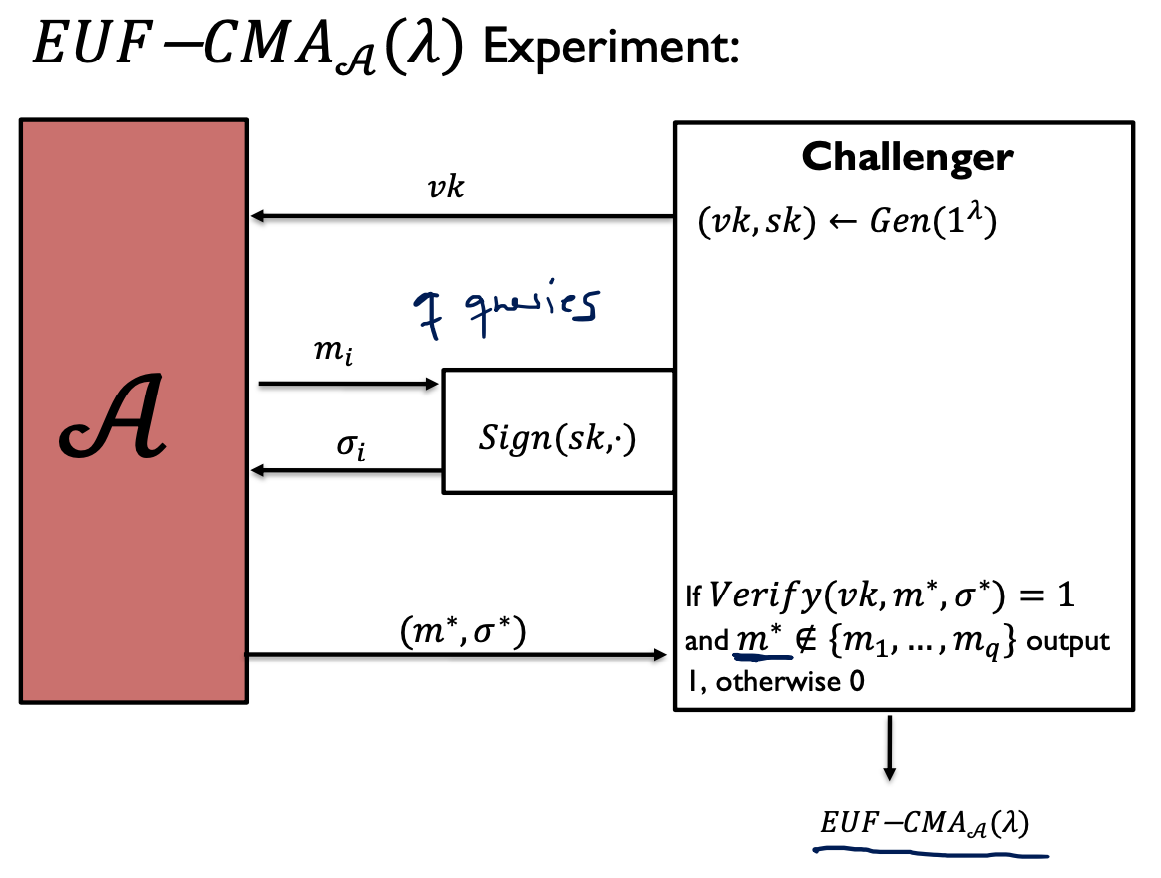
\includegraphics[width=160mm]{Graphics/Digital Signatures/ds3.png}
    \end{center}

\section{Applications: Certificates}
    \begin{itemize}
        \item How do you know you can trust a web-service?
        \item Certification Authority (CA) which certifies that someone can be trusted
        \item Trust in CA needs to be \textit{bootstrapped}
        \item X.509 Standard
    \end{itemize}
    \begin{center}
	    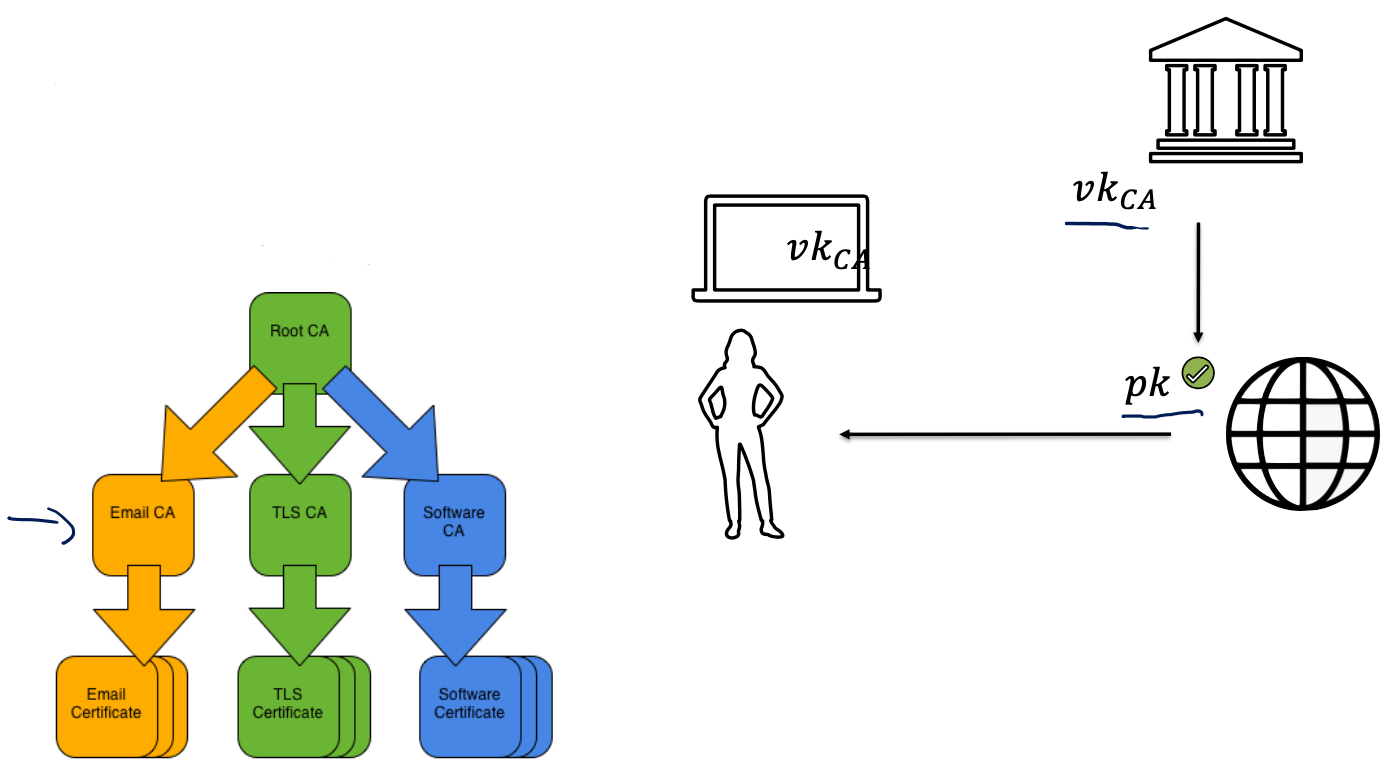
\includegraphics[width=160mm]{Graphics/Digital Signatures/ds4.png}
    \end{center}

\section{RSA Hash-and-Sign}
    \begin{itemize}
        \item We will now construct an EUF-CMA secure variant of the RSA signatures
        \item Idea: Hash message first, then sign
        \item Let $RSAGen$ be an RSA instance generation algorithm and $H: \{0,1\}^* \rightarrow \mathbb{Z}_N$ be a hash function
        \item The RSA Hash-and-Sign scheme $(Gen,Sign,Verify)$ is given as follows
        \begin{itemize}
            \item $Gen(1^{\lambda})$: Compute $(N,e,d) \leftarrow RSAGen(1^{\lambda})$.
            Output $vk \leftarrow (N,e)$ and $sk \leftarrow (N,d)$.
            \item $Sign(sk=(N,d),m)$: Compute and output $\sigma \leftarrow H(m)^d \ mod\ N$
            \item $Verify(vk=(N,e),m,\sigma)$: If $\sigma^e \ mod\ N = H(m) \ mod\ N$ output 1, otherwise 0.
        \end{itemize}
    \end{itemize}

\section{EUF-CMA Security}
    \begin{theorem}\label{thm9.1}
        \begin{itemize}
            \item Assume that the RSA assumption holds
            \item Assume further that $H$ is modeled as a random oracle
            \item Then $(Gen,Sign,Verify)$ is EUF-CMA secure
        \end{itemize}
    \end{theorem}
    \begin{proof}
        Assume towards contradiction that $\mathcal{A}$ is a PPT-adversary with non-negligible advantage $\epsilon$ against the $EUF-CMA$ security of $(Gen,Sign,Verify)$
        $$Pr[EUF-CMA_{\mathcal{A}}(\lambda)=1] > \epsilon$$
        \begin{center}
	        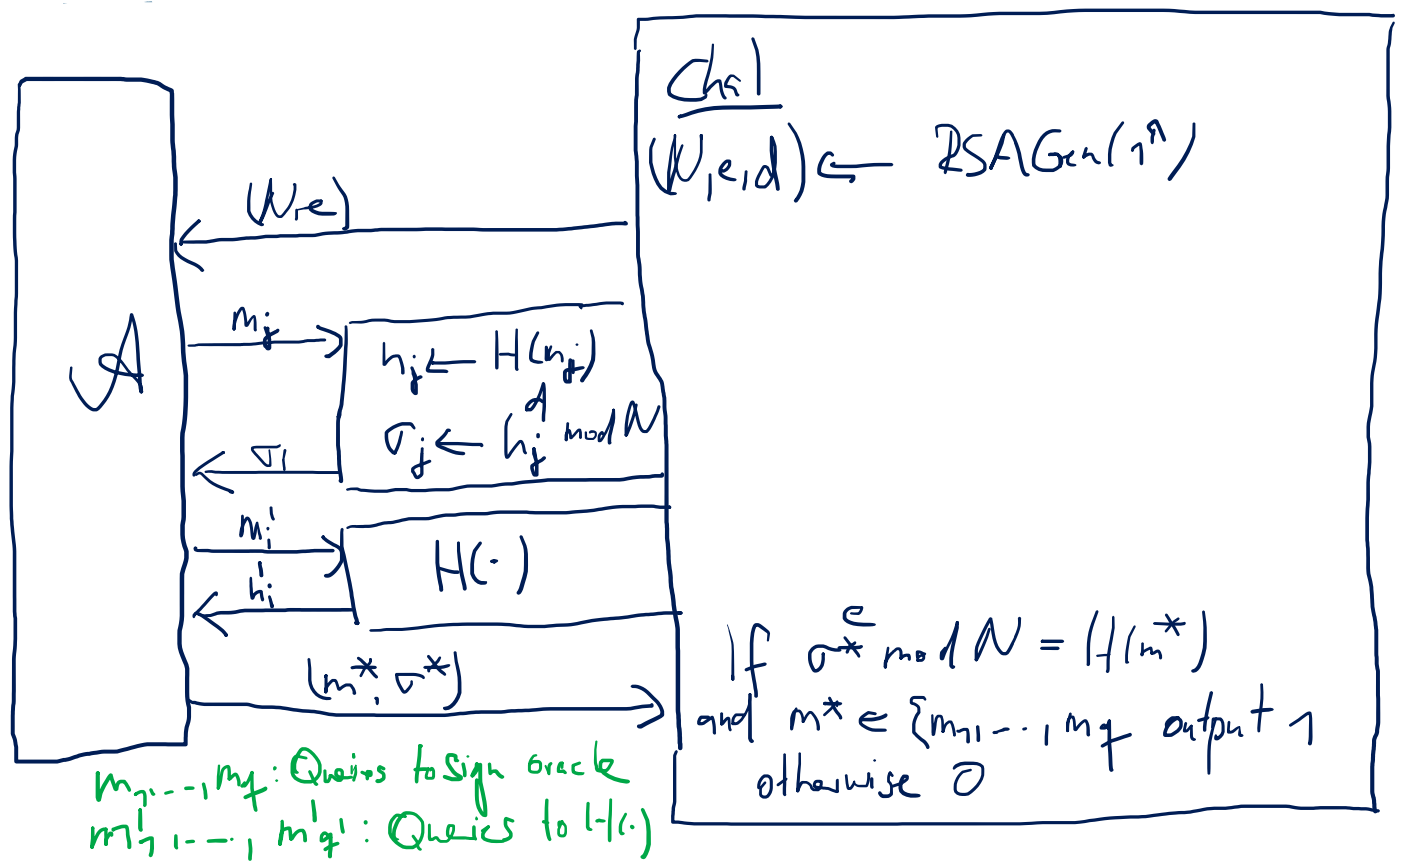
\includegraphics[width=160mm]{Graphics/Digital Signatures/ds5.png}
        \end{center}
        Let $m'_1,...,m'_{q'}$ be $\mathcal{A}$'s queries to $H(\cdot)$, where $q'=poly(\lambda)$.\\
        Define event $QUERIED$: $m^* \in \{m'_1,...,m'_{q'}\}$ (Forge-message)\\
        \textbf{Claim:} It holds that $Pr[EUF-CMA_{\mathcal{A}}(\lambda)=1 \mid \neg QUERIED] = \frac{1}{|\mathbb{Z}_N|} = negl(\lambda)$\\\\
        \textbf{Proof of Claim:}
            Recall that the random oracle $H(\cdot)$ is uniformly random and independent of everything else on positions on which it has not been queried yet.\\
            Thus, conditioned on $\neg QUERIED$, $H(m^*)$ is uniformly random in $\mathcal{A}$'s view
            $$Pr[H(m^*) = {\sigma^*}^2\ mod\ N \mid \neg QUERIED] = \frac{1}{|\mathbb{Z}_N|} < negl(\lambda)$$
            as $H(m^*)$ uniform in $\mathbb{Z}_N$ and thus the claim follows. It holds by LOTP
            \begin{align*}
                \epsilon < Pr[EUF-CMA_{\mathcal{A}}(\lambda)=1] &= Pr[EUF-CMA_{\mathcal{A}}(\lambda) \wedge QUERIED]\\
                        &+ \underbrace{Pr[EUF-CMA_{\mathcal{A}} \mid \neg QUERIED]}_{< negl.} \cdot \underbrace{Pr[\neg QUERIED]}_{\leq 1}
            \end{align*}
            $\Rightarrow Pr[EUF-CMA_{\mathcal{A}}(\lambda)=1 \wedge QUERIED] > \epsilon - negl(\lambda) = \epsilon'$ which is non-negligible.\\
            Observe that if $EUF-CMA_{\mathcal{A}}(\lambda) = 1$ and $QUERIED$ then there exist an index $\bar{i}$ such that $m^* = m'_{\bar{i}}$ and $H(m^*) = H(m'_{\bar{i}}) = {\sigma^*}^e \ mod\ N$\\
            We will now construct an adversary $\mathcal{A}$' which breaks the RSA assumption with probability $\frac{\epsilon'}{q'}$, which is non-negligible.
            \begin{center}
	            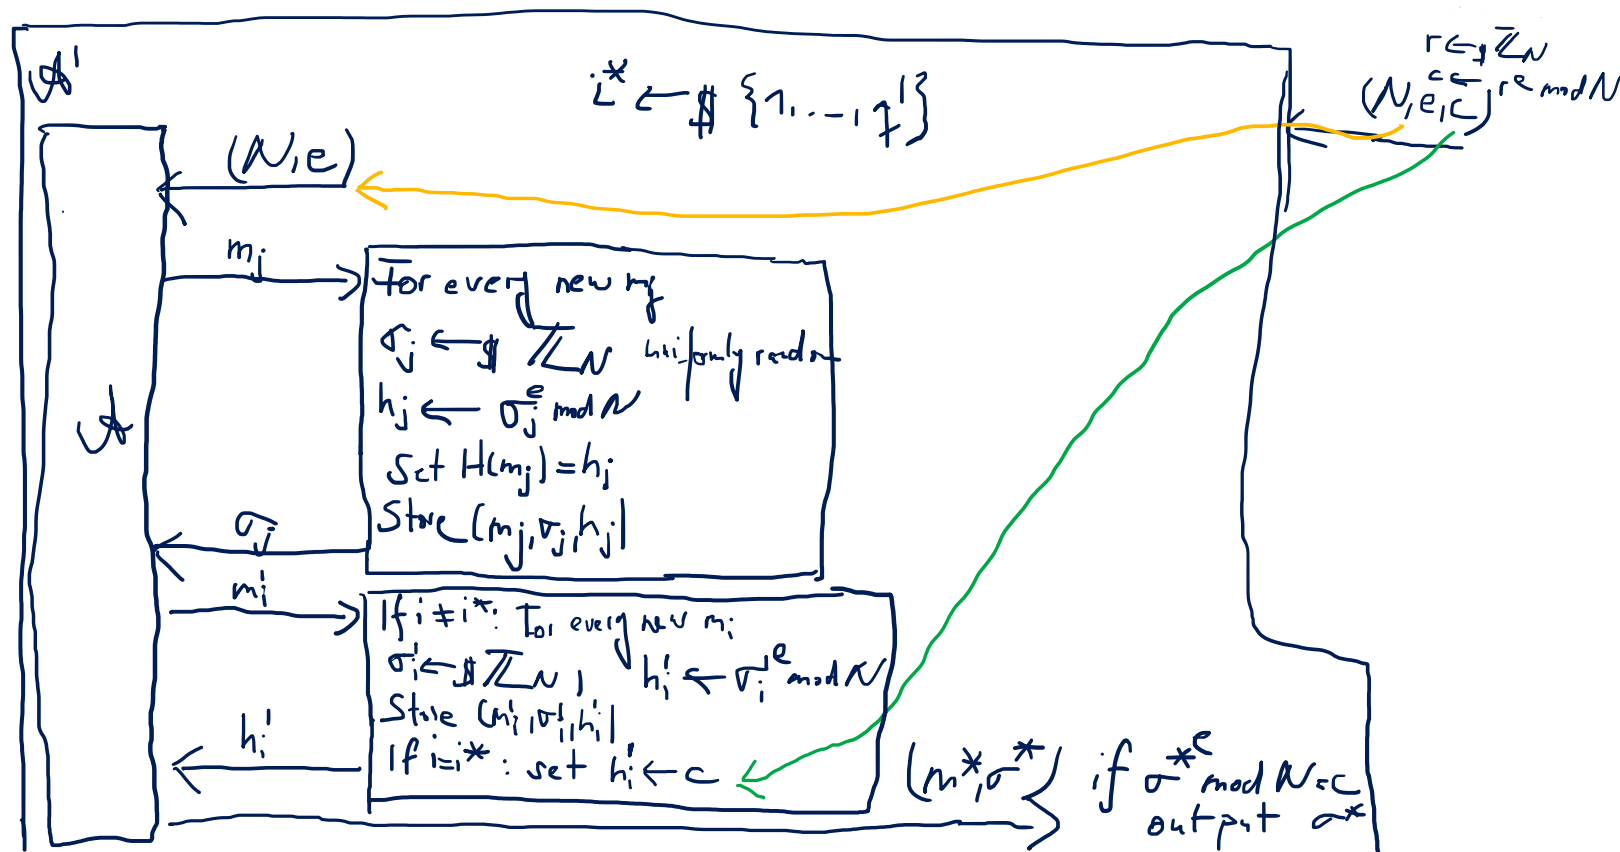
\includegraphics[width=160mm]{Graphics/Digital Signatures/ds6.png}
            \end{center}
            \textbf{Addition to figure:} If $\mathcal{A}$ queries Sign-oracle on $m'_{i^*}$ or has queried sign oracle on this value before, 
            $\mathcal{A}$' aborts an output $\bot$!\\
            From the view of $\mathcal{A}$, $\mathcal{A}'$ simulates the $EUF-CMA$ experiment faithfully.\\
            For every query $m_j$ it holds that $H(m_j) = \sigma^e_j \ mod\ N$ is distributed uniformly random as $\sigma_j$ is uniformly random in $\mathbb{Z}_N$
            and $x \mapsto x^e \ mod\ N$ is a permutation.\\
            $\Rightarrow Pr[i^* = \bar{i}] = \frac{1}{q'}$\\
            If $\mathcal{A}$ wins simulated $EUF-CMA$ experiment, $QUERIED$ and $i^* = \bar{i}$ then $\mathcal{A}$' wins RSA experiment.
            $$c = H(m_{i^*}) = H(m_{\bar{i}}) = H(m^*) = {\sigma^*}^e \ mod\ N$$
            \begin{align*}
                \Rightarrow Pr[Exp-RSA_{\mathcal{A}'}(\lambda) = 1] &\geq Pr[EUF-CMA_{\mathcal{A}}(\lambda) = 1 \wedge QUERIED \wedge i^* = \bar{i}]\\
                    &= \underbrace{Pr[EUF-CMA_{\mathcal{A}}(\lambda) = 1 \wedge QUERIED]}_{\geq \epsilon'} \cdot \underbrace{Pr[i^* = \bar{i}]}_{= \frac{1}{q'}} 
                    = \frac{\epsilon'}{q'}
            \end{align*}
            which is non-negligible.
            This contradicts the RSA assumption!
    \end{proof}

\section{Summary}
    \begin{itemize}
        \item Digital Signatures are the asymmetric version of message authentication codes
        \item Messages are signed using a secret signing key and can be verified using a public verification key
        \item Textbook RSA signatures have security issues
        \item Sensible security notion for signatures is EUF-CMA security, as for MACs
        \item RSA Hash-and-Sign is EUF-CMA secure in the random oracle model
    \end{itemize}


